\documentclass[10pt]{article}
\usepackage{fullpage}
\usepackage{graphicx}
\usepackage{amssymb}
\usepackage{epstopdf}
\usepackage{amsmath}
\usepackage{color,verbatim}
\usepackage{bm}
\usepackage{listings}
\usepackage{commath}
%\usepackage[framed,numbered,autolinebreaks,useliterate]{mcode}
%\usepackage{url,textcomp}
\DeclareGraphicsRule{.tif}{png}{.png}{`convert #1 `dirname #1`/`basename #1 .tif`.png}
\usepackage{float}
\usepackage[extreme]{savetrees}

\title{Approximation of a Gaussian}
\author{Brandon Gusto}
%\date{}                                           % Activate to display a given date or no date

\begin{document}

%\setlength{\baselineskip}{0.3cm}
%\linespread{0.75}

\begin{figure}
\center
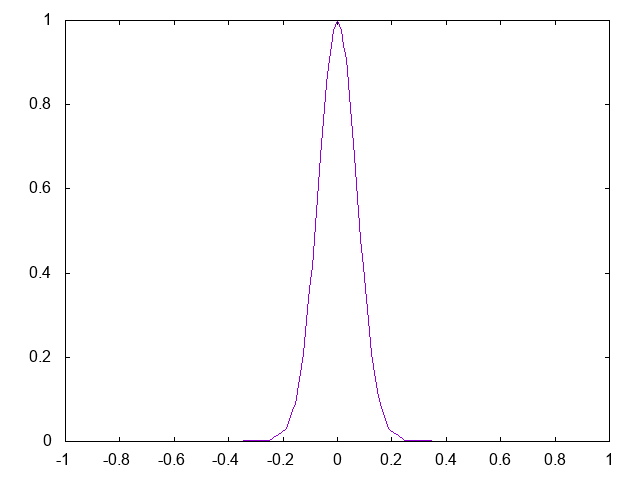
\includegraphics[scale=0.7]{solution10_minus2.png}
\caption{Gaussian function with $ \abs{d_{l}^{j}} > 10^{-2} $ }
\end{figure}

\begin{figure}
\center
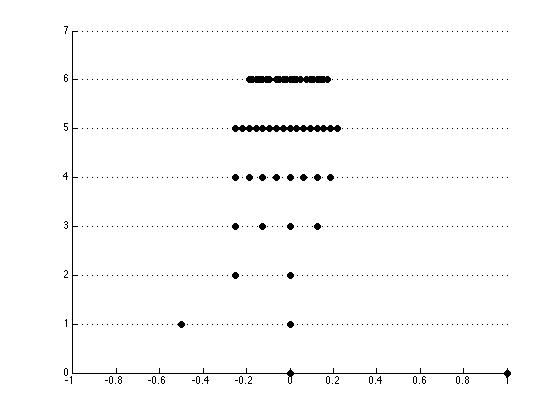
\includegraphics[scale=0.7]{5minus3_threshold.jpg}
\caption{Coefficients which are kept}
\end{figure}

\begin{figure}
\center
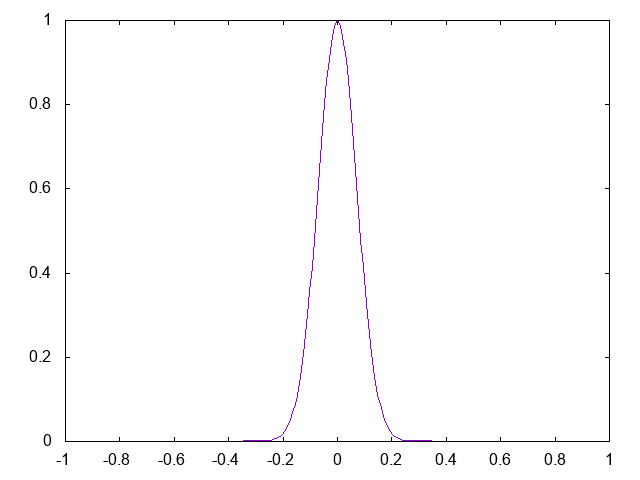
\includegraphics[scale=0.7]{solution10_minus3.png}
\caption{Gaussian function with $\abs{d_{l}^{j}} > 10^{-3} $ }
\end{figure}

\begin{figure}
\center
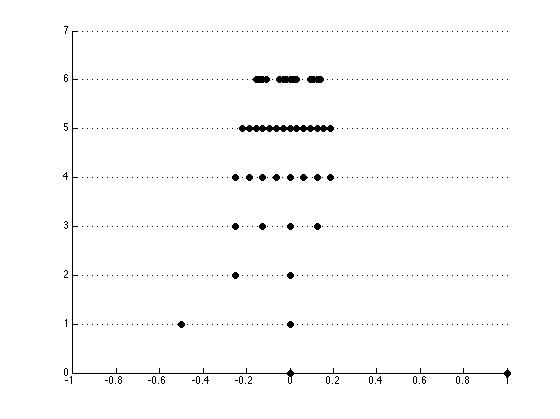
\includegraphics[scale=0.7]{minus3_threshold.jpg}
\caption{Coefficients which are kept}
\end{figure}

\end{document}